\documentclass{article}

\usepackage[final]{neurips_2025}

\usepackage[T1]{fontenc}
\usepackage[utf8]{inputenc}
\usepackage{hyperref}
\usepackage{url}
\usepackage{booktabs}
\usepackage{amsfonts}
\usepackage{nicefrac}
\usepackage{microtype}
\usepackage{xcolor}
\usepackage{graphicx}
\usepackage{amsmath,amssymb}
\usepackage{subcaption}

\title{GFlowNet-Guided Dropout Mask Sampling for Neural Bayesian Optimization}
\author{Anuar Aimoldin}
\date{}

\begin{document}
\maketitle

\begin{abstract}
This project studies whether learned dropout-mask generation improves neural Bayesian optimization over random mask sampling. The surrogate is a two-hidden-layer MLP trained with dropout, and the decision variable is a block-wise binary mask applied at inference time. The baseline samples masks uniformly at random, while the proposed method trains a contextual sequential GFlowNet to sample masks with probability proportional to a proxy improvement reward. To reduce implementation confounds, the refactored package pipeline uses shared per-step evaluation contexts, aligned training and inference mask semantics, and explicit diagnostics for reward reliability. I evaluate both methods on Branin (2D), Hartmann-6 (6D), and Ackley (10D). The main empirical result is mixed: random masks perform better on Branin and Hartmann-6, but the GFlowNet policy achieves lower final regret on Ackley-10. This suggests that learned mask generation is more promising in higher-dimensional settings, but reward quality and computational overhead remain central bottlenecks.
\end{abstract}

\section{Introduction}

Bayesian optimization (BO) is a standard framework for optimizing expensive black-box objectives under a limited evaluation budget \cite{snoek2012practical}. Classical BO uses a probabilistic surrogate, often a Gaussian process, together with an acquisition function that balances exploration and exploitation. In this project, I study a neural alternative in which the surrogate is a dropout MLP and uncertainty is represented through stochastic masked forward passes, following the Bayesian interpretation of dropout from \citet{gal2016dropout}.

The main question is whether mask sampling itself can be made more informative. Instead of treating dropout masks as undirected random perturbations, I model mask generation as a structured sampling problem and learn a distribution over masks with a GFlowNet \cite{bengio2023gflownet}. The hypothesis is that a learned mask policy should help more as the search space becomes larger and more multimodal. Recent work on GFlowOut shows that GFlowNets can represent useful distributions over dropout masks in supervised learning \cite{liu2023gflowout}; here I test the same idea inside a BO loop.

\section{Research Questions}

This study focuses on four questions:

\begin{enumerate}
    \item Can learned mask generation outperform random mask sampling for BO exploration?
    \item Are gains more visible on harder benchmarks, especially at higher dimensionality?
    \item How should the mask policy adapt as the dataset and surrogate change over BO iterations?
    \item Is the extra compute required for GFlowNet training justified by lower regret?
\end{enumerate}

\section{Method}

\subsection{Masked Neural Surrogate}

At BO iteration $t$, the observed dataset is
\[
\mathcal{D}_t = \{(x_i, y_i)\}_{i=1}^{n_t}, \qquad y_i = f(x_i).
\]

The surrogate is a two-hidden-layer MLP trained on normalized inputs and targets. Each hidden layer has dropout during training. At inference time, instead of sampling element-wise dropout, I use a \emph{block-wise} binary mask $m \in \{0,1\}^B$ that deterministically keeps or removes contiguous hidden blocks. A mask defines a masked predictor $\hat f_\theta(x; m)$.

\subsection{Proposal Generation from a Mask}

Given a finite candidate set $\mathcal{C}_t$, each mask induces a proposed point
\[
x_m = \arg\max_{x \in \mathcal{C}_t} \hat f_\theta(x; m).
\]

To estimate whether the proposal is promising, I evaluate $x_m$ under a held-out ensemble of random masks $h_1,\dots,h_H$. This produces a proxy mean and standard deviation,
\[
\tilde\mu(x_m) = \frac{1}{H}\sum_{j=1}^H \hat f_\theta(x_m; h_j),
\qquad
\tilde\sigma(x_m) = \mathrm{Std}\big[\hat f_\theta(x_m; h_j)\big].
\]

Let $y_t^{\mathrm{best}}$ be the best observed oracle value so far. The proxy improvement score is
\[
\Delta(m) = \tilde\mu(x_m) + \beta \tilde\sigma(x_m) - y_t^{\mathrm{best}},
\]
which is then converted into a positive reward $R(m)$ used for mask sampling. In the original implementation this conversion used a fixed softplus transform. In the refactored package pipeline, reward scaling is treated as an explicit protocol choice, with raw, normalized, and rank-based variants available as controlled alternatives. This change is important because it turns reward construction from a hidden implementation detail into an experimental axis that can be stress-tested directly. Across all variants, the underlying objective is the same: reward masks that both predict high value and preserve some uncertainty through the held-out ensemble.

\subsection{Random Baseline vs. GFlowNet Policy}

The two compared policies differ only in how masks are generated:

\begin{itemize}
    \item \textbf{Random baseline:} sample block-wise masks uniformly at random, evaluate each sampled mask with $R(m)$, and query the proposal from the best mask in the sampled set.
    \item \textbf{GFN policy:} train a sequential GFlowNet so that $P(m \mid c_t) \propto R(m)$, then draw candidate masks from this learned policy and again query the proposal from the best sampled mask.
\end{itemize}

The GFlowNet generates masks one block at a time and is conditioned on a context vector $c_t$ computed from the current dataset. In the implementation, $c_t$ contains BO progress, normalized response statistics, input dispersion, and the benchmark dimension. This is a simple way to address non-stationarity as the BO loop evolves.

\section{Experimental Setup}

I evaluate the method on the three baselines requested in the project prompt:

\begin{itemize}
    \item Branin (2D), converted to maximization by optimizing $-\mathrm{Branin}(x)$,
    \item Hartmann-6 (6D),
    \item Ackley (10D), converted to maximization by optimizing $-\mathrm{Ackley}(x)$.
\end{itemize}

The main metric is simple regret,
\[
r_t = f^\star - \max_{i \le t} f(x_i),
\]
where $f^\star$ is the known benchmark optimum. Each experiment is run over 5 random seeds.

\begin{table}[t]
\centering
\caption{Benchmark-specific BO configurations used in the executed config-driven runs.}
\label{tab:configs}
\small
\begin{tabular}{lcccccc}
\toprule
Benchmark & Dim & $n_{\text{init}}$ & BO iters & Hidden dim & Candidate pool & GFN steps \\
\midrule
Branin & 2 & 8 & 18 & 64 & 2048 & 160 \\
Hartmann-6 & 6 & 14 & 22 & 96 & 4096 & 180 \\
Ackley & 10 & 20 & 24 & 128 & 4096 & 200 \\
\bottomrule
\end{tabular}
\end{table}

Across all benchmarks, each BO step compares 96 sampled masks for the random policy and 96 sampled masks for the GFlowNet policy. The proxy reward uses 24 held-out random masks. All experiments were executed in the \texttt{general\_env} conda environment.

\subsection{Implementation Controls in the Refactored Pipeline}

A substantial part of the project effort went into reducing ambiguity about whether the observed performance differences came from the method itself or from the surrounding implementation. The refactored \texttt{pkg} pipeline therefore introduces three controls that are important for interpreting the final results.

First, all mask evaluations within a BO step now share the same candidate pool and the same held-out mask ensemble. This removes a major source of evaluation noise present in a naive implementation, where each mask could otherwise be scored against a different randomly drawn context. Second, the mask semantics used during surrogate training and during inference-time mask search are aligned, so that the policy is no longer optimized over a mask space that differs substantially from the one seen by the surrogate during learning. Third, the pipeline logs reward reliability diagnostics in addition to regret: step-wise reward variance, improvement variance, floor-reward frequency, same-mask repeat-evaluation variance, and the correlation between proxy improvement and realized oracle gain.

These controls do not guarantee that the proxy reward is perfectly calibrated, but they make the resulting conclusions more defensible. In particular, if a mixed or negative result persists after these implementation changes, it is less plausible to dismiss it as a simple artifact of noisy reward evaluation or an avoidable mismatch between training and inference.

\section{Results}

\begin{table}[t]
\centering
\caption{Final performance over 5 seeds. Lower regret is better.}
\label{tab:final_results}
\small
\begin{tabular}{lccc}
\toprule
Benchmark & Random final regret & GFlowNet final regret & Better method \\
\midrule
Branin (2D) & $1.7813 \pm 1.1734$ & $2.1459 \pm 0.7910$ & Random \\
Hartmann-6 (6D) & $0.5571 \pm 0.3059$ & $0.7027 \pm 0.5144$ & Random \\
Ackley (10D) & $18.1526 \pm 1.1661$ & $16.7447 \pm 1.5421$ & GFlowNet \\
\bottomrule
\end{tabular}
\end{table}

Table~\ref{tab:final_results} shows a clear mixed pattern. On the lower-dimensional benchmarks, learned mask generation did not outperform the random baseline. On Branin, the random policy finished with a lower mean regret by $0.3646$. On Hartmann-6, the gap in favor of random masks was smaller, $0.1456$, but the same qualitative conclusion held. Ackley-10 was different: here the GFlowNet policy improved final regret by $1.4079$, providing the strongest positive evidence for the method.

\begin{figure*}[t]
    \centering
    \begin{subfigure}[t]{0.32\textwidth}
        \centering
        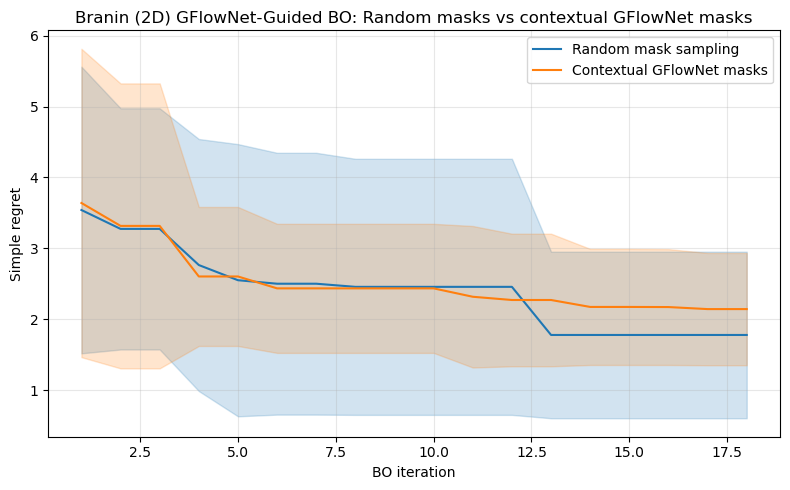
\includegraphics[width=\textwidth]{img/branin_regret_comparison.png}
        \caption{Branin (2D)}
    \end{subfigure}
    \hfill
    \begin{subfigure}[t]{0.32\textwidth}
        \centering
        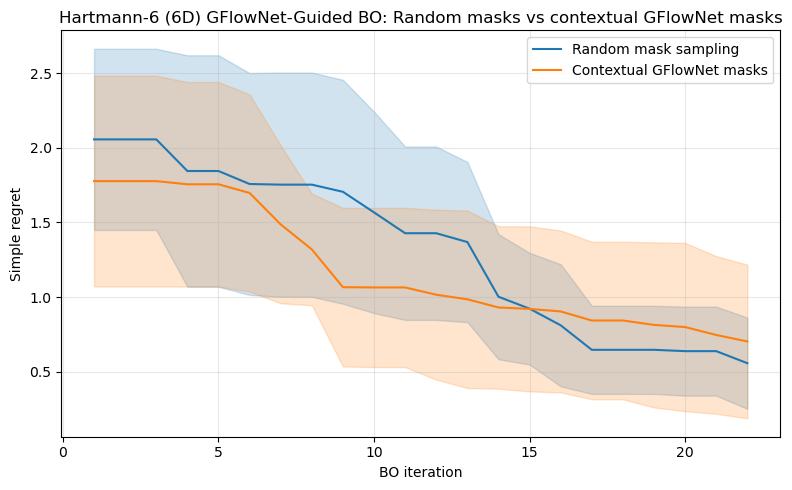
\includegraphics[width=\textwidth]{img/hartmann6_regret_comparison.png}
        \caption{Hartmann-6 (6D)}
    \end{subfigure}
    \hfill
    \begin{subfigure}[t]{0.32\textwidth}
        \centering
        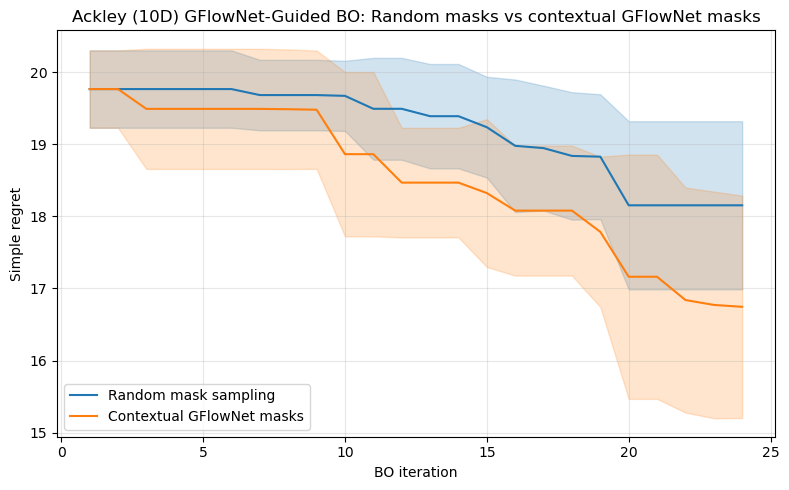
\includegraphics[width=\textwidth]{img/ackley10_regret_comparison.png}
        \caption{Ackley (10D)}
    \end{subfigure}
    \caption{Mean simple regret over BO iterations. Shaded regions denote one standard deviation across 5 seeds. Random mask sampling is stronger on Branin and Hartmann-6, while the contextual GFlowNet policy is stronger on Ackley-10.}
    \label{fig:regret_comparisons}
\end{figure*}

Figure~\ref{fig:regret_comparisons} makes the trend visible over the full optimization horizon. On Branin and Hartmann-6, the random baseline remains competitive throughout the run. On Ackley-10, the GFlowNet curve overtakes the random baseline and ends at a lower regret, suggesting that the learned policy becomes more useful as the search problem becomes harder.

\begin{figure*}[t]
    \centering
    \begin{subfigure}[t]{0.48\textwidth}
        \centering
        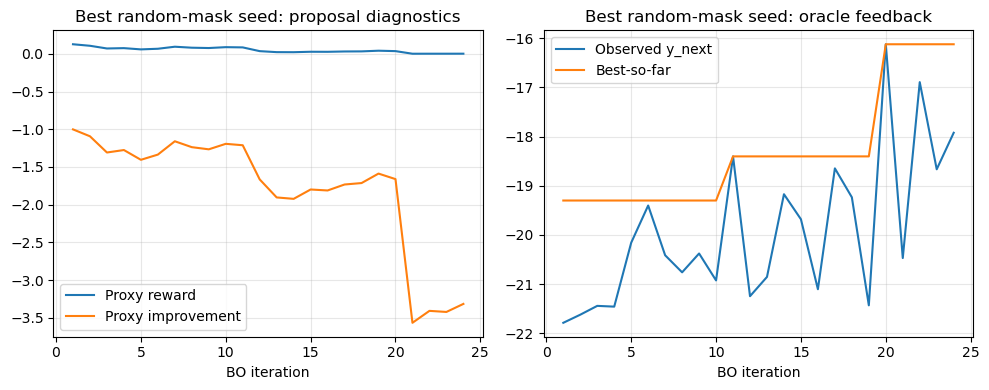
\includegraphics[width=\textwidth]{img/ackley10_random_diagnostics.png}
        \caption{Best random-mask seed on Ackley-10}
    \end{subfigure}
    \hfill
    \begin{subfigure}[t]{0.48\textwidth}
        \centering
        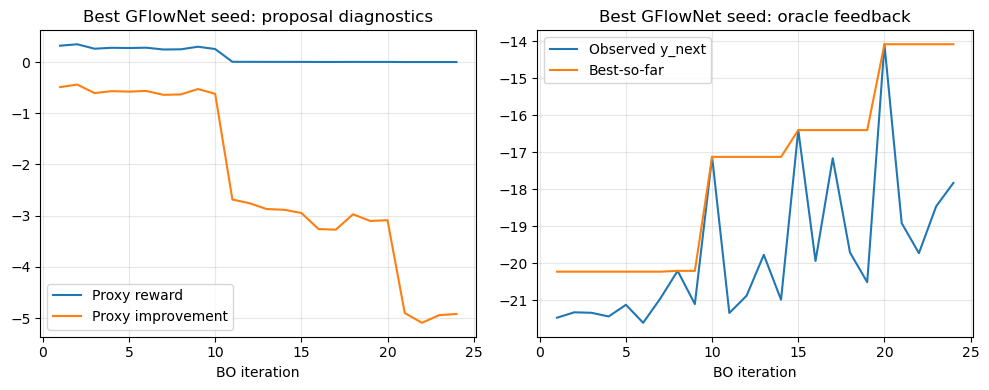
\includegraphics[width=\textwidth]{img/ackley10_gfn_diagnostics.png}
        \caption{Best GFlowNet seed on Ackley-10}
    \end{subfigure}
    \caption{Proposal diagnostics for Ackley-10. Each plot shows proxy reward and proxy improvement together with the actual queried oracle value and best-so-far trajectory. The GFlowNet run achieves stronger final best-so-far performance, which matches the lower final regret reported in Table~\ref{tab:final_results}.}
    \label{fig:ackley_diagnostics}
\end{figure*}

The Ackley diagnostics in Figure~\ref{fig:ackley_diagnostics} are useful because they correspond to the only benchmark where the learned policy produced a clear benefit. They show that the best GFlowNet seed converts high proxy scores into a stronger best-so-far trajectory than the best random baseline seed. This does not prove that the reward is perfectly aligned with oracle improvement, but it shows that the reward is at least sometimes good enough to help in a harder, higher-dimensional setting.

\subsection{Compute Trade-off}

Because GFlowNet-guided BO adds a learned mask-policy training loop inside each BO iteration, the wall-clock overhead is an important part of the result rather than an implementation detail. I therefore ran a separate timing experiment with the same benchmark configurations and seeds used for the main results. Table~\ref{tab:compute_tradeoff} compares mean final regret with mean wall-clock time per trial.

\begin{table}[t]
\centering
\caption{Compute trade-off over 5 seeds. Positive regret gain means GFlowNet achieved lower regret than the random baseline.}
\label{tab:compute_tradeoff}
\small
\begin{tabular}{lcccccc}
\toprule
Benchmark & Random regret & GFN regret & Random time & GFN time & Slowdown & Regret gain \\
\midrule
Branin & $1.7813$ & $2.1459$ & $3.75$s & $128.07$s & $34.11\times$ & $-0.3646$ \\
Hartmann-6 & $0.5571$ & $0.7027$ & $5.77$s & $310.73$s & $53.85\times$ & $-0.1456$ \\
Ackley & $18.1526$ & $16.7447$ & $7.52$s & $509.42$s & $67.70\times$ & $1.4079$ \\
\bottomrule
\end{tabular}
\end{table}

The compute trade-off is severe. On Branin and Hartmann-6, the GFlowNet policy is both slower and worse. In those settings, the extra computation is clearly not justified. Ackley-10 is the only benchmark where the additional training cost buys a measurable optimization benefit: GFlowNet improves mean final regret by $1.4079$, but it does so while increasing mean wall-clock time per trial from $7.52$ seconds to $509.42$ seconds. This makes Ackley-10 a meaningful positive result, but also shows that the current method is far from cost-effective.

\begin{table}[t]
\centering
\caption{Mean per-iteration runtime breakdown in seconds. The dominant extra cost comes from GFlowNet training, not surrogate fitting.}
\label{tab:runtime_breakdown}
\small
\begin{tabular}{lcccccc}
\toprule
Benchmark & Random surrogate & Random proposal & GFN surrogate & GFN train & GFN proposal & Total GFN iter \\
\midrule
Branin & $0.08$ & $0.13$ & $0.08$ & $6.84$ & $0.19$ & $7.11$ \\
Hartmann-6 & $0.09$ & $0.17$ & $0.09$ & $13.73$ & $0.30$ & $14.12$ \\
Ackley & $0.10$ & $0.21$ & $0.10$ & $20.77$ & $0.35$ & $21.23$ \\
\bottomrule
\end{tabular}
\end{table}

Table~\ref{tab:runtime_breakdown} explains where the overhead comes from. Surrogate training time is almost identical between methods across all benchmarks, so the baseline neural BO loop itself is not the bottleneck. The additional cost comes overwhelmingly from the inner GFlowNet optimization, which grows from roughly $6.8$ seconds per BO iteration on Branin to $20.8$ seconds on Ackley-10. Proposal selection is slightly more expensive for GFlowNet than for random masks, but this difference is small compared with the cost of training the policy. This confirms that future work should focus on reducing the amount of GFlowNet optimization needed per BO step, or on learning a reward that produces larger regret gains so that the overhead is easier to justify.

\section{Discussion}

The main conclusion is that the current evidence supports a \emph{conditional} version of the project hypothesis rather than a universal one. Learned mask generation is not yet a clear replacement for random mask sampling on simple benchmarks. However, the positive result on Ackley-10 suggests that a learned policy can become useful when dimensionality increases and the search landscape becomes more difficult.

The results also clarify the key bottlenecks:

\begin{itemize}
    \item \textbf{Reward alignment:} the method depends heavily on the quality of the proxy improvement reward. If the surrogate is overconfident, the GFlowNet can learn to prefer masks that exploit this bias rather than produce genuinely informative BO proposals.
    \item \textbf{Non-stationarity:} the policy is trained inside a changing BO loop, so the reward landscape over masks shifts at every iteration. The contextual conditioning used here is a first step, but it is probably not sufficient.
    \item \textbf{Compute cost:} the learned policy is expensive. The dedicated timing experiment shows $34\times$ to $68\times$ wall-clock slowdown relative to the random baseline, with most of the extra time spent on GFlowNet training rather than surrogate fitting.
\end{itemize}

The refactored implementation also changes how these results should be interpreted. In the earlier monolithic prototype, it was reasonable to worry that reward noise, inconsistent evaluation contexts, or train/inference mask mismatch might dominate the comparison. The new package pipeline does not remove all sources of approximation error, but it does remove the most obvious implementation confounds and exposes them through targeted diagnostics. As a result, a negative or mixed outcome now carries more scientific weight: it is closer to evidence about the method, rather than just evidence about a brittle script.

These observations are still scientifically useful. Even the negative results on Branin and Hartmann-6 are informative because they narrow down the conditions under which GFlowNet-guided mask generation seems worth pursuing. Just as importantly, they now do so under a cleaner and more reproducible experimental protocol.

\section{Conclusion}

This report presented an implementation of GFlowNet-guided dropout mask sampling for neural Bayesian optimization and compared it against a matched random-mask baseline on Branin, Hartmann-6, and Ackley-10. The final result is mixed: random masks remain better on the two lower-dimensional benchmarks, while the GFlowNet policy improves regret on Ackley-10. After refactoring the codebase into a controlled package pipeline with shared per-step evaluation contexts, aligned mask semantics, and explicit reward diagnostics, the most defensible conclusion is not simply that the method sometimes works and sometimes fails. It is that the remaining mixed evidence is substantially more trustworthy because the main implementation-level confounds were explicitly addressed.

The next technical priorities are to improve proxy-reward calibration, test stronger contextual conditioning or periodic retraining strategies, and expand the benchmark suite so the dependence on dimensionality and multimodality can be measured more systematically. A second priority is to report the new implementation diagnostics and ablations directly alongside regret curves, so that future iterations of the project can distinguish more sharply between reward-design limitations and genuine limits of GFlowNet-guided mask search.

\appendix

\section{Additional Diagnostic Plots}

Figures~\ref{fig:branin_diagnostics_appendix} and~\ref{fig:hartmann_diagnostics_appendix} show the same proposal diagnostics as in the Ackley case, but for the Branin and Hartmann-6 benchmarks. These plots help explain the negative results in the main table: on both lower-dimensional tasks, the learned mask policy does not convert high proxy scores into better final best-so-far trajectories than the random baseline.

\begin{figure*}[t]
    \centering
    \begin{subfigure}[t]{0.48\textwidth}
        \centering
        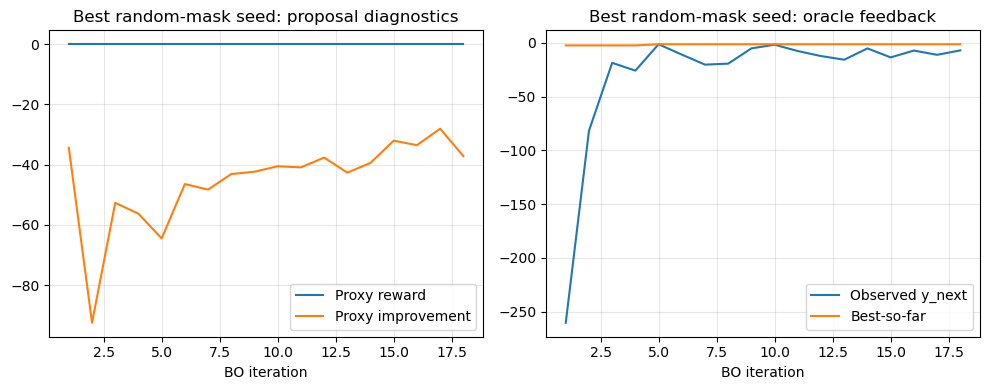
\includegraphics[width=\textwidth]{img/branin_random_diagnostics.png}
        \caption{Best random-mask seed on Branin}
    \end{subfigure}
    \hfill
    \begin{subfigure}[t]{0.48\textwidth}
        \centering
        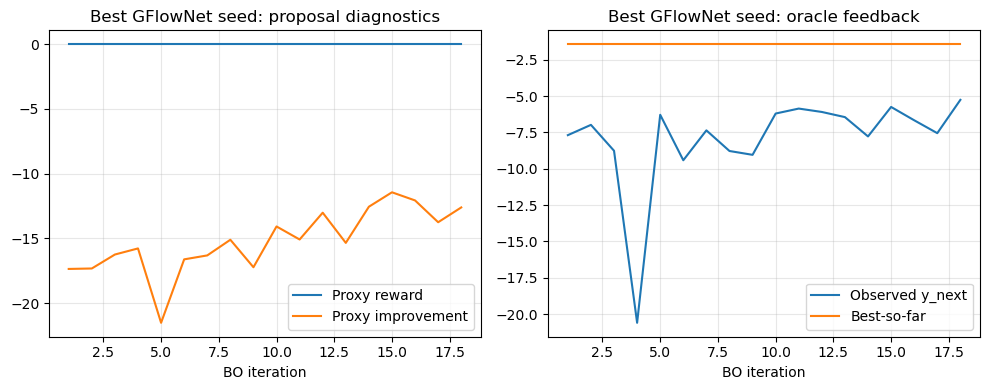
\includegraphics[width=\textwidth]{img/branin_gfn_diagnostics.png}
        \caption{Best GFlowNet seed on Branin}
    \end{subfigure}
    \caption{Branin proposal diagnostics. The random baseline still converts sampled proposals into a better final best-so-far value than the learned policy, despite the GFlowNet run being somewhat more consistent across seeds.}
    \label{fig:branin_diagnostics_appendix}
\end{figure*}

\begin{figure*}[t]
    \centering
    \begin{subfigure}[t]{0.48\textwidth}
        \centering
        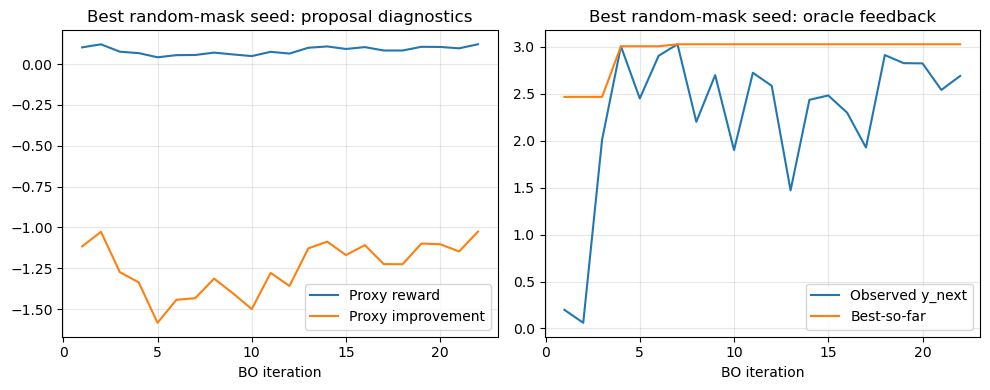
\includegraphics[width=\textwidth]{img/hartmann6_random_diagnostics.png}
        \caption{Best random-mask seed on Hartmann-6}
    \end{subfigure}
    \hfill
    \begin{subfigure}[t]{0.48\textwidth}
        \centering
        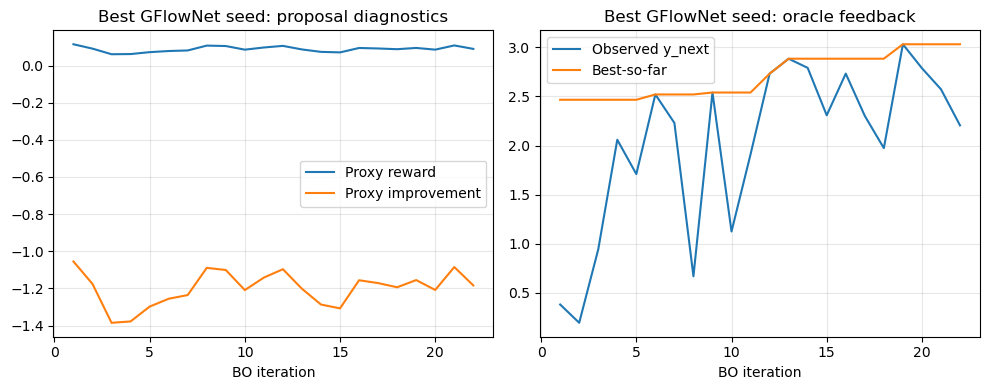
\includegraphics[width=\textwidth]{img/hartmann6_gfn_diagnostics.png}
        \caption{Best GFlowNet seed on Hartmann-6}
    \end{subfigure}
    \caption{Hartmann-6 proposal diagnostics. The learned policy remains viable, but its proxy-driven proposals do not translate into lower final regret than random mask sampling in this benchmark.}
    \label{fig:hartmann_diagnostics_appendix}
\end{figure*}

\bibliographystyle{plainnat}
\bibliography{references}

\end{document}
